% PLEASE USE THIS FILE AS A TEMPLATE
% Check file iosart2c.tex for more examples
%
% Journal:
%   Journal of Ambient Intelligence and Smart Environments (jaise)
%   Web Intelligence and Agent Systems: An International Journal (wias)
%   Semantic Web: Interoperability, Usability, Applicability (SW)
% IOS Press
% Latex 2e

% options: jaise|wias|sw
% add. options: [seceqn,secfloat,secthm,crcready,onecolumn]


%\documentclass{iosart2c}

\documentclass[sw]{iosart2c}
%\documentclass[wias]{iosart2c}
%\documentclass[jaise]{iosart2c}
\usepackage{flushend}
\usepackage[T1]{fontenc}
\usepackage{times}%
\usepackage{natbib}
%\usepackage[dvips]{hyperref}
\usepackage{amsmath}
\usepackage{dcolumn}
%\usepackage{endnotes}
\usepackage{graphics}

\usepackage{url}
\usepackage{array}

\usepackage[utf8]{inputenc} % please use UTF8 encoding
%\usepackage[round]{natbib}

\usepackage{mathptmx}       % selects Times Roman as basic font
%\usepackage{helvet}         % selects Helvetica as sans-serif font
\usepackage{courier}        % selects Courier as typewriter font
%\usepackage{type1cm}        % activate if the above 3 fonts are
                            % not available on your system
%
\usepackage{graphicx}        % standard LaTeX graphics tool
                             % when including figure files
\usepackage{multicol}        % used for the two-column index
%\usepackage[bottom]{footmisc}% places footnotes at page bottom

% see the list of further useful packages
% in the Reference Guide

\usepackage{graphicx}



\newcommand{\lemon}{\emph{lemon}}
%\newcommand{\myremark}[2]{{\textbf{\marginpar{$\parallel$}(* \textit{#1:} #2 *)}}}
%\newcommand{\jmc}[1]{\myremark{John}{#1}}
%\newcommand{\pc}[1]{\myremark{Philipp}{#1}}
%\newcommand{\emp}[1]{\myremark{Elena}{#1}}
%\newcommand{\emp}[1]{\myremark{JEK}{#1}}

\pubyear{0000}
\volume{0}
\firstpage{1}
\lastpage{1}

% choose options for [] as required from the list
% in the Reference Guide


\begin{document}

\newcommand{\imgpath}{.}
\newcommand{\onto}[1]{\texttt{#1}}
\newcommand{\word}[1]{\textsl{#1}}

\begin{frontmatter}

%\pretitle{}
\title{\emph{le\-mon\-U\-by} - a large, interlinked, syntactically-rich lexical resource for ontologies}
%\runningtitle{Lemon $+$ Uby 4 MLODE-Postproc}
%\subtitle{}

%\review{}{}{}

% Two or more authors:
\author[A]{\fnms{Judith} \snm{Eckle-Kohler},\thanks{Corresponding author, http://www.ukp.tu-darmstadt.de}}
%\thanks{Do not use capitals for the author's surname.}},
\author[B]{\fnms{John Philip} \snm{M\textsuperscript{c}Crae}}
and
\author[C]{\fnms{Christian} \snm{Chiarcos}}
\runningauthor{Eckle-Kohler et al.}
\address[A]{Ubiquitous Knowledge Processing (UKP) Lab,  Department of Computer Science,  Technische Universit{\"a}t Darmstadt
and Information Center for Education, German Institute for International Educational Research, Germany, 
http://www.ukp.tu-darmstadt.de}
\address[B]{Cognitive Interaction Technology (CITEC), Semantic Computing Group, Universit\"at Bielefeld, Germany, http://www.sc.cit-ec.uni-bielefeld.de}
\address[C]{Applied Computational Linguistics (ACoLi), Department of Computer Science and Mathematics, Goethe-University Frankfurt am Main, Germany, 
http://acoli.cs.uni-frankfurt.de}
%\address[C]{}}
%\address[D]{}}

%\institute{John McCrae \at CITEC, Universit\"at Bielefeld, \email{jmccrae@cit-ec.uni-bielefeld.de} \and ...}

%\maketitle

\begin{abstract}
We introduce \emph{le\-mon\-U\-by}, a new lexical resource integrated in the Semantic Web
%\footnote{\url{http://www.lemon-model.net/lexica/uby/}}
which is
 the result of converting data extracted from the existing large-scale linked lexical resource UBY to
 the \emph{lemon} lexicon model.
 The following data from UBY were converted: WordNet, FrameNet, VerbNet,
English and German Wiktionary, the English and German
entries of Ome\-ga\-Wi\-ki,
as well as links between pairs of these lexicons at the word sense level (links between VerbNet and FrameNet,
VerbNet and WordNet, WordNet and FrameNet, WordNet and Wiktionary, WordNet and German Ome\-ga\-Wiki).
We linked  \emph{le\-mon\-U\-by} to other lexical resources and linguistic
terminology repositories in the Linguistic Linked Open Data cloud and outline possible applications of this new dataset.

%Pairs of these resources are linked at the sense level, and in addition, \emph{le\-mon\-U\-by} is
%first, there are linkings to other lexical resource in the LLOD cloud, and second, we established a linking of
%POS categories in UBY to -the OLiA reference model. lemonUBY is an important enrichment of the Semantic Web, as it is
%a resource which is rich in verbs and provides fine-grained linguistic information on verbs.
% We report on the large-scale population of the \emph{lemon} lexicon model by a subset of UBY lexical resources
% and describe the resulting data set which we call \emph{lemonUBYlite}.
% The mapping of the UBY-LMF lexicon model to \emph{lemon} is discussed as well as the actual conversion of
% UBY lexical resources to \emph{lemon}.
% Furthermore, two kinds of linkings of \emph{lemonUBYlite} to the LLOD cloud are performed: first,
% a linking of POS values in \emph{lemonUBYlite} to OLiA, and second, a linking of the \emph{lemonUBYlite} WordNet
%  to a WordNet in the LLOD cloud.
\end{abstract}

\begin{keyword}
Lexicon model\sep lemon\sep UBY-LMF\sep UBY\sep OLiA \sep ISOcat \sep  WordNet \sep VerbNet \sep FrameNet  \sep Wiktionary \sep Ome\-ga\-Wi\-ki
\end{keyword}

\end{frontmatter}

%%%%%%%%%%% The article body starts:

% \renewcommand{\lemon}{\index{lemon}\emph{lemon}}
%

\section{Introduction}

\noindent Recently, the language resource community has begun to explore the opportunities offered by the Semantic
Web, lead by the formation of the Linguistic Linked Open Data (LLOD) cloud
and an increasing interest in making use of Linked Open Data principles in the context
of Natural Language Processing (NLP) and Linguistics  \cite{chiarcos2012linked}.
The use of RDF supports data integration and offers a large body of tools for accessing this data.
Furthermore, the linked data approach gives rise to novel research questions in the context of
language resources and their application.

 For lexical resources, data integration has been in
 the focus of interest for many years, resulting in numerous mappings and linkings of lexica, as well as
standards for representing lexical resources, such as the ISO 24613:2008 Lexical Markup Framework
(LMF) \cite{francopoulo2006lexical}. In this context, the LLOD cloud can be considered as a new data integration platform, enabling
linkings not only between lexical resources, but also between lexical resources and
other language resources.

We extend the LLOD cloud by a new lexical resource called \emph{le\-mon\-U\-by}\footnote{\url{http://www.lemon-model.net/lexica/uby/}}
which is
 the result of converting data extracted from the existing large-scale linked lexical resource UBY
 \cite{gurevych2012uby}\footnote{\url{http://www.ukp.tu-darmstadt.de/uby/}} to
 the \emph{lemon} lexicon model.
UBY has been developed independently from Semantic Web technology. It is LMF based
and a subset of the LMF-compliant UBY lexicons is pairwise linked at the word sense level.
The \emph{lemon} lexicon model has been developed for lexical resource integration on the Semantic Web
\cite{mccrae2012interchanging}.
This lexicon model serves as a common interchange format for lexical resources on the Semantic Web
and has been designed to represent and share lexical resources that are linked to ontologies, i.e., ontology lexica.
Making use of a lexicon interchange format, such as \emph{lemon} is not only important for data integration,
but also for the reuse of lexicons.


% A particularly large-scale example of lexical resource integration is the
% lexical-semantic resource UBY \cite{gurevych2012uby}\footnote{\url{http://www.ukp.tu-darmstadt.de/uby/}}.
% UBY has been developed independently from Semantic Web technology and linked data principles.
% UBY is
% \begin{itemize}
%  \item based on LMF, i.e., all lexicons integrated in UBY have been standardized according to the lexicon model
% UBY-LMF \cite{ecklekohler2012uby,TUD-CS-2013-0003}, which is an instantiation of the abstract ISO standard LMF,
% \item a linked lexical resource, i.e., a subset of the UBY lexicons is pairwise linked at the word sense level.
% \end{itemize}
%
% For lexical resource integration on the Semantic Web, the \emph{lemon} lexicon model has been developed \cite{mccrae2012interchanging}.
% This lexicon model serves as a common interchange format for lexical resources on the Semantic Web
% and has been designed to represent and share lexical resources that are linked to ontologies, i.e., ontology lexica.
% Making use of a lexicon interchange format, such as \emph{lemon} is not only important for data integration,
% but also for the reuse of lexicons.

While many lexical resources have already been included in the LLOD cloud, e.g.,
\cite{Bizer_Lehmann_Kobilarov_Auer_Becker_Cyganiak_Hellmann_2009, mccrae2012integrating, navigli2012babelnet, de2008language, deMeloWeikum2008c},
the LLOD cloud is still missing a
large-scale lexical resource rich in lexical information on
verbs, including aspects such as syntactic behaviour and 
semantic roles of a verb's arguments.
%how semantic arguments of verbs can be realised syntactically. 
Such information is crucial for lexicalizing relational knowledge%
%which is often expressed by using verbs %% CC: slightly redundant
, e.g., the relation $like(Experiencer, Theme)$ can be lexicalized syntactically with a verb as in "NP likes NP".

%There has also been some work towards the integration of FrameNet \cite{baker1998berkley} to the Semantic Web \cite{narayanan2003framenet}.
%All these resources provide a substantial body of lexical knowledge, including semantic relations, multilingual
%information and encyclopedic knowledge.

The new resource \emph{le\-mon\-U\-by} addresses this gap: Along with resources for word-level semantics (WordNet \cite{fellbaum98-wordnet}, 
English and German Wiktionary,\footnote{\url{http://www.wiktionary.org}} and the English and German entries of 
Ome\-ga\-Wi\-ki,\footnote{\url{http://www.omegawiki.org}}) we converted two syntactically rich resources from
UBY to the \emph{lemon} format: FrameNet \cite{baker1998berkley} and VerbNet \cite{kipper2008large}. %% CC: list all converted resources here
For further data integration, we established links between \emph{le\-mon\-U\-by} and other language resources in the LLOD cloud.

% We address this gap by converting data from the existing lexical resource UBY to the \emph{lemon} format.
% The following data from UBY were converted: WordNet, FrameNet, VerbNet \cite{kipper2008large},
% English and German Wiktionary~\footnote{\url{http://www.wiktionary.org}}, the English and German
% entries of Ome\-ga\-Wi\-ki~\footnote{\url{http://www.Ome\-ga\-Wi\-ki.org}},
% as well as links between pairs of these lexicons at the word sense level (links between Verb\-Net--Frame\-Net,
% Verb\-Net--Word\-Net, Word\-Net--Frame\-Net, Word\-Net--Wiktionary, Word\-Net -- German Ome\-ga\-Wiki).
% We call the resulting lexical resource \emph{le\-mon\-U\-by}\footnote{\url{http://www.lemon-model.net/lexica/uby/}}
% and established links between \emph{le\-mon\-U\-by} and oher language resources in the LLOD cloud.

% The data-set presented in this paper, \emph{le\-mon\-U\-by}, is the result of
% converting a selection of UBY lexica to
% the \emph{lemon} format:
% it contains interoperable and interlinked versions of WordNet, FrameNet,
% VerbNet \cite{kipper2008large}, English and German Wiktionary~\footnote{\url{http://www.wiktionary.org}},
%  and the English and German entries of
% Ome\-ga\-Wi\-ki~\footnote{\url{http://www.Ome\-ga\-Wi\-ki.org}}.


%Such information is crucial for lexicalizing relational knowledge which is typically expressed
%by using verbs along with specific arguments.


%In the current LLOD cloud, large-scale lexical resources rich in encyclopedic knowledge, such as DBPedia, are
%predominant, while
%the size and diversity of lexical resources rich in linguistic knowledge, particularly for verbs,
% is limited so far.
% There has already been some work towards the integration of FrameNet \cite{baker1998berkley} to the Semantic Web \cite{narayanan2003framenet},
%as well as WordNet
%\cite{van2006conversion}, WordNet and Wiktionary\cite{mccrae2012integrating}, and recently BabelNet as a multilingual
%lexical resource integrating WordNet and Wikipedia \cite{navigli2012babelnet}.
% In the Semantic Web, several versions of WordNet REF
%and FrameNet REF have been available as linked data for quite same time, but due to the LLOD movement
%new resources such as
%Wiktionary REF and BabelNet REF have been added just recently.
%However, the LLOD cloud contains no large-scale lexical resource yet, which is rich in lexical information on
%verbs, including aspects such as their syntactic behavior and how semantic arguments of verbs can be realized
%syntactically. Such information is crucial for lexicalizing relational knowledge which is typically expressed
%by using verbs along with specific arguments.

%  To summarize, our contributions are threefold: (i) an RDF version of data extracted from the existing lexical resource
%  UBY (called \emph{le\-mon\-U\-by}),
% (ii) a mapping of the lexicon model UBY-LMF to \emph{lemon}, and (iii)
% linkings of \emph{le\-mon\-U\-by} to other language resources in the LLOD cloud.

%Moreover, the
%format chosen for the RDF versions of FrameNet and WordNet
% was specific to the underlying data model of these two resources which have been characterized as
%complementary by \cite{Baker:2009}.
%However, the LLOD cloud contains no large-scale lexical resource yet which is rich in lexical information on
%verbs, including aspects such as their syntactic behavior and how semantic arguments of verbs can be realized
%syntactically. Such information is crucial for lexicalizing relational knowledge which is typically expressed
%by using verbs along with specific arguments.
%The dataset \emph{le\-mon\-U\-by} which we present in this paper addresses these gaps:
%it contains interoperable and interlinked versions of WordNet [FEL 98], FrameNet [BAK 98],
%VerbNet [KIP 08], and multilingual Ome\-ga\-Wi\-ki (www.Ome\-ga\-Wi\-ki.org).
%\emph{le\-mon\-U\-by} is linked to the LLOD cloud and has a number of
%additional features that add significant value to the LLOD cloud. We will describe these features and the creation
%of this dataset in the following sections.

 \section{Representing lexical-semantic resources as Linked Data: \emph{lemon}}

\begin{figure}
 \begin{center}

 	 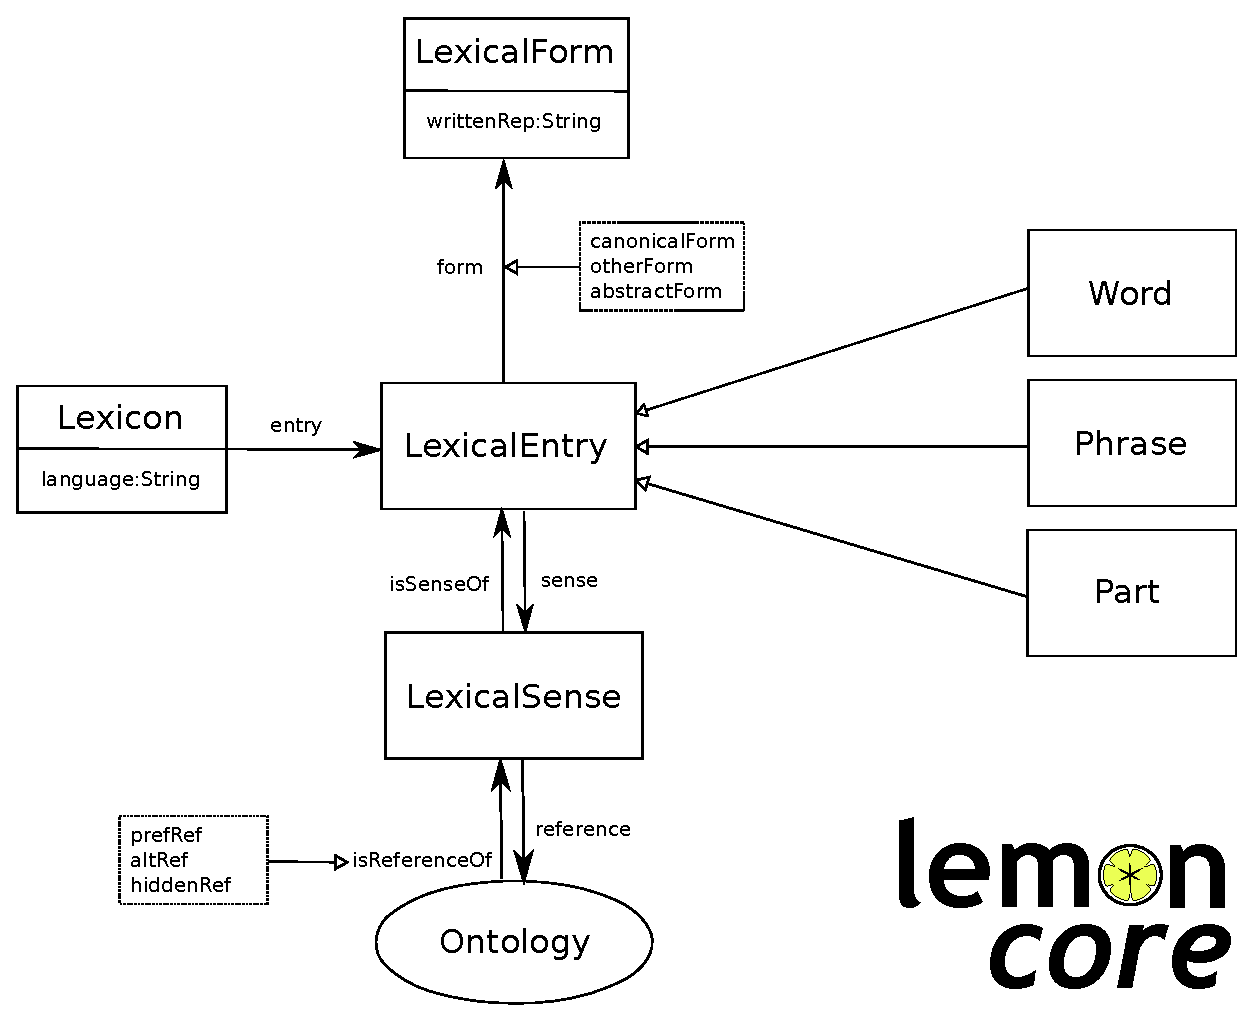
\includegraphics[width=1.0\columnwidth]{images/lemon-core}

 \end{center}
\caption{The core of the \emph{lemon} model\label{lemon-core}}
\end{figure}

\noindent 
There has been significant work towards integrating lexical resources using RDF and
Semantic Web principles~\cite{chiarcos2011towards}, and many resources are already
available as Linked Data. %% CC: less redundant
    % Many lexical resources have already been included in the LLOD cloud, e.g., WordNet, Wikipedia
    % (DBpedia \cite{Bizer_Lehmann_Kobilarov_Auer_Becker_Cyganiak_Hellmann_2009}),
    % and Wiktionary, as well as integrated resources, such as an integrated version of WordNet and Wiktionary\cite{mccrae2012integrating},
    % or of  WordNet and Wikipedia (BabelNet, \cite{navigli2012babelnet}, lexvo?).
    %There has also been some work towards the integration of FrameNet \cite{baker1998berkley} to the Semantic Web \cite{narayanan2003framenet}.
    %All these resources provide a substantial body of lexical knowledge, including semantic relations, multilingual
    %information and encyclopedic knowledge.
Yet, representing lexical resources in RDF does not per se make them semantically
interoperable. Consider, for instance, existing conversions of WordNet and FrameNet \cite{van2006conversion,narayanan2003framenet},
where a simple mapping to RDF is provided, and augmented with OWL semantics so that reasoning could be applied to the structure of the resource.
However, the formats chosen for the RDF versions of WordNet and FrameNet are specific to the underlying data models of WordNet and FrameNet.
    % CC: originally, this sentence mentioned WordNet only, which doesn't make sense as we explicitly announced that we would talk about both WordNet and FrameNet
Although these lexicons are complementary resources~\cite{baker2009wordnet}, % CC: slightly simplified
it is difficult (i) to link them in this form on the Semantic Web, and (ii) to use them as interchangeable modules in NLP applications.

% notably the conversion of WordNet
% \cite{van2006conversion}. They provided a simple mapping from WordNet to RDF, and
% augmented it with OWL semantics so that reasoning could be applied to the structure of the resource.
% Similarly, there has been some work towards mapping
% FrameNet \cite{baker1998berkley} to RDF \cite{narayanan2003framenet}.
% However, the formats chosen for the RDF versions of WordNet and FrameNet are specific to the underlying data models of WordNet
% and FrameNet. Since these lexicons have
% been characterised as complementary resources~\cite{baker2009wordnet}, it is difficult (i) to link the existing versions
% on the Semantic Web, and (ii) to use them as interchangeable modules in NLP applications.

%this resource was specific to the underlying data model of WordNet.
In order to overcome this difficulty, the \emph{lemon} model \cite{mccrae2012interchanging} was proposed
as a common interchange format for lexical resources on the Semantic Web.
\emph{lemon} has its historical roots in LMF and thus allows 
    %% CC: "having roots in" is not causal, merely circumstantial, hence, not "to allow"
easy conversion from LMF-like, non-linked data resources. 
    %% CC: From a SW perspective, one could simply call these "legacy resources", but I guess Judith wouldn't like that too much ;)
It links to data categories in
  annotation terminology repositories, and most of all,
  it realises a separation of lexicon and ontology layers, so that \emph{lemon} lexica can be linked to existing ontologies
in the linked data cloud.


% that supports publishing
% lexical-semantic resources as linked data on the basis of the following principles:
%
% \begin{description}
% \item[LMF-based]: To allow easy conversion from non-linked data resources.
% \item[RDF-native]: Publishing as linked data, with RDFS and OWL used to describe
%   the semantics of the model.
% \item[Modular]: Separation of lexicon and ontology layers, so that \emph{lemon} lexica can be linked to existing ontologies
% in the linked data cloud.
% \item[Externally defined data categories]: Linking to data categories in
%   annotation terminology repositories, rather than being limited to a specific part-of-speech tag set.
% \item[Principle of least power]: The smaller the model and the less expressive the language,
% 	the wider its adoption and the higher the reusability of the
% 	data\cite{shadbolt2006semantic}.
% \end{description}

This core model is illustrated in Fig.\ \ref{lemon-core}, which defines the
basic elements used by all lexica published as linked data. In addition to this there
are a number of modules used to model linguistic description, syntax, morphology
and relationships between lexica.\footnote{More detail of the model and descriptions of
the modules can be found at \url{http://lemon-model.net}}

\emph{lemon} has been used as a basis for integrating the data of the
English Wiktionary
    % \footnote{A (human-readable) dictionary created along wiki principles, see \url{http://www.wiktionary.org}} 
    %% CC: has been introduced in Sect. 1 already
with
the RDF version of WordNet \cite{mccrae2012integrating}.
\emph{lemon}'s similarity
to the WordNet model made this conversion straight-forward, with only the need for
a slight change in modelling to accommodate inflectional variants of lexical
entries.


 \section{Large-scale integration of lexical-semantic resources: UBY and UBY-LMF}

%\begin{verbatim}
%JEK: describe uby-lmf lexicon model and uby data
%mapping to lemon -> JEK, JM
%- sense in lemon vs sense in UBY-LMF
%\end{verbatim}
% it is important to keep separate the different levels:
% the standard: LMF (an abstract standard, not directly usable)
% the lexicon model: UBY-LMF vs lemon
% the format: XML vs RDF (vs RelaxNG ...)

\noindent
UBY is both a network of interlinked lexical-semantic resources
and a project on continuous integration and linking of lexical resources for NLP applications.
 It is motivated by the
observation that an essential requirement in NLP is the availability of a wide range of lexical resources that
can be used for many different NLP tasks. In a continuous process, such resources
are integrated into UBY by means of (i) making them interoperable  and (ii)
linking them to other resources in UBY at the sense level.

%UBY has currently integrated 10 LRs in two languages, see www.ukp.tu-darmstadt.de/uby. Only 8 of these LRs have open licenses and
%can be offered as a UBY database dump for download: English WordNet, Wiktionary, Wikipedia, FrameNet and VerbNet, German Wikipedia, Wiktionary, and multilingual OmegaWiki.
%A subset of these LRs is linked at the word sense level and these sense alignments are open as well.
%There are monolingual sense alignments between VerbNet--FrameNet\footnote{\url{http://verbs.colorado.edu/semlink/}} and
%VerbNet--WordNet\footnote{\url{http://verbs.colorado.edu/~mpalmer/projects/verbnet}} as well as between WordNet--Wikipedia \cite{niemann2011peoples} and WordNet--Wiktionary  \cite{meyer2011what}. In addition, Uby provides cross-lingual sense alignments between WordNet and the German OmegaWiki \cite{gurevych2012uby}, also including the inter-language links already given in Wikipedia and OmegaWiki.
%
%UBY databases can be created according to specific application needs: a user might want to use only a subset of the LRs integrated into UBY, convert them to UBY-LMF and import them into
%a database. Any UBY database can be accessed with a single Java-API which is continuously developed along with the conversion tools in an Open Source Project on Google Code (code.google.com/p/uby).
%UBY and UBY-LMF are CC-licensed and the UBY-related software is licensed under the open Apache license.

In UBY, interoperability is achieved by standardizing lexical resources according
to UBY-LMF \cite{ecklekohler2012uby,TUD-CS-2013-0003}, a lexicon
model which is an instantiation of 
    % the ISO standard %% CC: redundant with sect. 1
LMF, specifically designed for NLP.
%instantiates the Lexical Markup Framework (LMF, ISO 24613:2008, \cite{francopoulo2006lexical}).
The lexicon model UBY-LMF has been developed to fully cover a wide range of heterogeneous lexical resources
without information loss, which resulted in a fine-grained model of lexical information types (documented by
data categories from ISOcat,\footnote{\url{http://www.isocat.org/}} 
 the implementation of the ISO 12620:2009 Data Category Registry)
 and was accompanied by
an extension of the ISO standard LMF by a few elements.
The extensibility of UBY-LMF was a primary design principle in order to enable the integration of further 
(in particular automatically acquired) lexical resources. %% , in the future. %% CC: wann sonst ;)

% JEK the use of Data Category Registry such as ISOcat is part of the LMF standard, so it is not necessary to add this here
% (UBY-LMF is an instantiation of LMF), and second, regarding data categories from
% ISOcat -- they are used as comments for li
% it uses externally defined data categories from
% ISOcat as comments.\footnote{\url{http://www.isocat.org/rest/dcs/484}}
%\begin{description}
%\item[Principle of Adoption]: UBY-LMF has been designed to fully cover a wide range of heterogeneous lexical resources
%without information loss.
%This resulted  in a fine-grained model of lexical information types, which ranges from morphology and lexical syntax to lexical semantics and the mapping between syntactic and semantic arguments.
%jmc: Note really sure that this is possible, at any rate lemon covers most things and unlike LMF allows arbitrary extensions

%\item[Independence of implementation]: UBY-LMF  is independent of any particular implementation. There are many ways to implement an LMF lexicon model \cite{francopoulo2007lexical}, including RDF.
% jmc: LMF makes assumptions of an underlying XML model, lemon of an RDF model, both can be mapped to XML, JSON, SQL etc.
%\end{description}


% UBY-LMF has been implemented in two ways: first, as a DTD, and second,
% as a Java Object-Relational Mapping by means of the Hibernate framework\footnote{\url{http://www.hibernate.org}},
% which allows mapping any instance of UBY-LMF either to a SQL database or to an XML file.
%Both ways of representing UBY-LMF do not require the use of globally unique identifiers (URIs).
%However, an implementation of UBY-LMF in RDF would be possible as well.
%For instance, an implementation of LMF to include URIs has been suggested by \cite{francopoulo2007lexical}.
%, since UBY-LMF as such is independent of any particular implementation or
%serialization and an LMF lexicon model can be implemented in many ways \cite{francopoulo2007lexical}.

% JEK I would not call it extension
%An extension of LMF to include URIs \cite{Francopoulo2007}, and full-fledged RDF linearizations of LMF have been suggested, e.g., in the context of the Lexicon Model for Ontologies (Lemon) as described by McCrae et al. (2011)\nocite{McCrae2011}.
% An implementation of LMF to include URIs has already been suggested\cite{francopoulo2007lexical}.
% In fact, providing lexical resources, in particular interlinked resources such as UBY, as linked data is a very natural
% step to take and
% allows us to integrate UBY-LMF-based resources with other resources previously converted to RDF.
%e.g., in the context of the developing Semantic Web.

The mapping from UBY-LMF to \emph{lemon} is motivated by an increase in interoperability with the Semantic Web and its resources, thereby making it available to a new group of potential users and novel applications. %% CC: to motivate the conversion in explicit words
Beyond this, mapping UBY-LMF to \emph{lemon} is an interesting task per se, because \emph{lemon} links lexical resources and
ontologies, whereas UBY-LMF is not related to any ontology. Another benefit is that LMF is not an open standard (in the sense that its specification is not freely available), while \emph{lemon} % provides an interchange format which %% CC: shorter
fully complies with open data and open access principles.

%An extension of LMF to include URIs \cite{Francopoulo2007}, and full-fledged RDF linearizations of LMF have been suggested, e.g., in the context of the Lexicon Model for Ontologies (Lemon) as described by McCrae et al. (2011)\nocite{McCrae2011}.

%Originally, Uby was implemented using the Lexical Markup Framework, a standard aiming for interoperability among lexical-semantic resources.

% LMF is no format, it is an abstract standard
%First, the LMF standard is not an open standard (in the sense that its specification is not freely available), and,
% according to the experience of UBY, the application of the standard requires % making
%NLP domain-specific modifications to the abstract model defined by the standard.
%Second, the currently used implementation of UBY-LMF does not consider how resources can be uniquely identified on the web.


%and in its frequently used
% LMF does not say anything about serialization, XML is just an illustrative example
 %serialization as XML, it does not consider how resources can be uniquely identified on the web.
%Furthermore, according to the experience of UBY, application of the standard requires % making
%NLP domain-specific modifications to the standard schema.

%An RDF formalization tackles %of LMF allows us to tackle
%some of these problems, and this has been suggested by the LMF developers themselves% \citep{francopoulo2009multilingual}
%.\footnote{\url{http://www.tagmatica.fr/lmf/LMF_revision_14_In_OWL29october2007.xml}}

%LMF is grounded in earlier research on feature structures (i.e., directed acyclic graphs) that have been suggested as a generalization over resource-specific data structures \citep{veronis-ide92-feature-structures-for-lexical-dbs}.
%Feature structures are a flexible and general formalism, which became the basis for subsequent standardization, in particular, in LMF.
%\citealp{francopoulo2006lexical}).

% LMF represents a metamodel % aiming to provide a standard
% to represent semantic information in NLP lexicons and machine-readable dictionaries.
% It has been successfully applied to develop resources, including the different Uby data sets.

%Converting a lexical resource in UBY-LMF format to lemon requires a mapping of the UBY-LMF lexicon model to the lemon lexicon model.

% Although both UBY-LMF and \emph{lemon} are based on LMF, the mapping revealed substantial differences which are mainly due to the fact that
% \emph{lemon} is a model for ontology lexica where the lexicon and ontology layers are kept separate. Thus, sense representations in \emph{lemon} primarily consist of references to the associated ontology
% where a rich and domain-specific sense definition is provided.
% The development of UBY-LMF, on the other hand, has been driven by the requirement to cover a large variety of
%  lexical information types, which ranges from morphology and lexical syntax to lexical semantics and the mapping between syntactic and semantic arguments.
% Thus, the resulting lexicon model makes use of very fine-grained sense specifications which are often grounded in linguistic theories,
% e.g. Frame Semantics (the basis of FrameNet) or the Levin alternation classes of verbs \cite{levin93} (the basis of VerbNet).
%

 % UBY-LMF, UBY, mapping of UBY-LMF to lemon
 \section{Converting UBY lexica to  \emph{lemon}: \emph{le\-mon\-U\-by}}

\noindent 
To automatically convert data from UBY-LMF (extracted from UBY) to  \emph{lemon},
we performed a mapping of UBY-LMF elements to \emph{lemon} concepts and properties.
    % CC: from sect. 3
This involves two aspects: Formalizing and mapping UBY data structures in a Semantic-Web compliant way,
and the actual conversion of UBY data. 

\subsection{Modeling Data Categories: \emph{ubyCat}}

\noindent 
In UBY-LMF, most of the terms used and many features (e.g., the feature ``partOfSpeech'' and the corresponding attribute values)
are linked to % standardized %% CC: N�, ISOcat ist standardisiert, nicht der Inhalt
%% JEK Inhalt und Form lassen sich schwer trennen ;) - aber ich wei� was du meinst
community-maintained data categories in ISOcat.\footnote{\url{http://www.isocat.org/rest/dcs/484}}
As the mapping of UBY-LMF to \emph{lemon} preserves this linking, \emph{le\-mon\-U\-by}
is linked to ISOcat as well.
The content of ISOcat is also available as Linked Data \cite{ldl-windhouwer}, 
% actually, it isn't in the cloud diagram, for the reasons mentioned below -- and neither should be GOLD, for the same reasons. 
%But for GOLD, there is at least an implicit note on the website that the content provided should be available
and therefore, provides a possible and direct way to interconnect \emph{le\-mon\-U\-by} with other LLOD resources 
at the level of linguistic data categories.

% not relevant any more (ISOcat will have an open license)
% However, ISOcat does currently not contain an explicit license statement, even though its content is available over the internet.
% While people involved (Menzo Windhouwer, p.c., June 2012) believe that a publication under
% an open license would be appreciated, it has not been clarified whether the
% restrictive licensing policy of the ISO that applies to the ISOcat technical
% specifications also extends to the ISOcat data categories.
% A similar problem persists with the General Ontology of Linguistic Description \cite[GOLD]{farrar2003markup}
% %(GOLD)
% \footnote{\url{http://linguistics-ontology.org/}}, another LLOD-linked % this is true, at least from OLiA
% terminology repository.
%Currently, GOLD does not contain
%an explicit license statement as well, but it is available on-line, and as a community
%project,
%publication under an open license can be expected.

However, ISOcat is not a formal ontology, but only a semistructured collection of terms, and while it serves as a 
repository of definitions, it does not provide a formal data model that can be applied to a resource: 
ISOcat contains doublets created by different data providers, %e.g., VoiceProperty [DC-3551] vs. voice [DC-1433], 
and such superficially similar categories may actually have incompatible definitions, e.g., gerundive [DC-1294] is an ``adjective formed from a verb'' (excluding verbal nouns), whereas gerundive [DC-2243] is a ``non-finite form (...) other than the infinitive'' (including verbal nouns). Hierarchical relations between ISOcat terms are possible, but not obligatory, and when compared with a full-fledged ontology, ISOcat terms that represent superconcepts for a bundle of features (e.g., ActiveVoice [DC-3064] dcif:isA VoiceProperty [DC-3551]) do not distinguish relational and categorial aspects: VoiceProperty could be either a property that assigns ActiveVoice to a particular unit of annotation, or a concept that defines the range of such a relation.

To render UBY/ISOcat data categories in a formal data model, we created the OWL/DL 
ontology \emph{ubyCat}\footnote{\url{http://purl.org/olia/ubyCat.owl}} which defines the semantics of
linguistic terms used in \emph{le\-mon\-U\-by}:
With respect to \emph{data structures}, it extends the \emph{lemon} ontology,\footnote{\url{http://www.monnet-project.eu/lemon}} concepts 
that are equivalent with \emph{lemon} but have a different label are included, flagged as deprecated (and not used during the conversion),
but left in the ontology to help UBY-LMF users find the equivalent \emph{lemon} categories. 

With respect to \emph{data categories}, \emph{ubyCat} is linked to the Ontologies of Linguistic Annotations
(OLiA) \cite{chiarcos2008ontology,chiarcos2012ontologies},\footnote{\url{http://purl.org/olia}} a modular 
architecture of OWL/DL ontologies that link resource-specific linguistic terminology (as for UBY) to an overarching
`Reference Model' which (a) provides a particular view on linguistic terminology, and (b) serves as an interface to
multiple community-maintained terminology repositories such as ISOcat with which it is linked. Details of this
linking are described in Sect.\ \ref{sec-olia}.

\subsection{Converting the Data}

\noindent
The actual conversion  of UBY data was achieved by means of
an XML style sheet transform\footnote{The XSL file can be downloaded at
\url{https://raw.github.com/jmccrae/lemon.api/master/src/main/resources/xslt/ubylmf2lemon.xsl}}
that implements a mapping of the UBY-LMF model to the \emph{lemon} model.

The following data from UBY were converted: WordNet, FrameNet, VerbNet,
English and German Wiktionary, the English and German
entries of Ome\-ga\-Wi\-ki,
as well as links between pairs of these lexicons at the word sense level:

\begin{itemize}
 \item monolingual manual sense links for
VerbNet--Frame\-Net,\footnote{\url{http://verbs.colorado.edu/semlink/}}
VerbNet--WordNet,\footnote{\url{http://verbs.colorado.edu/~mpalmer/projects/verbnet}} and 
automatic sense links for WordNet--Frame\-Net \cite{tonelli-pighin:2009:CoNLL,laparra-rigau:2009:RANLP09},
and WordNet--Wiktionary \cite{meyer2011what};
\item cross-lingual automatic sense links between WordNet and German Ome\-ga\-Wiki \cite{gurevych2012uby}, and manual inter-language links
already given in Ome\-ga\-Wi\-ki.
\end{itemize}
%% CC: slightly shortened

The resulting resource \emph{le\-mon\-U\-by} has been published at
\url{http://lemon-model.net/lexica/uby}
under an open CC-BY-SA license. The choice of a share-alike
license was due to UBY being published under the same license.
Statistics for
the \emph{le\-mon\-U\-by} resources including the sense links within this dataset
are given in table \ref{triples}. An obvious gap is the 
German Wiktionary which is currently not linked to any other resource within
\emph{le\-mon\-U\-by}. Future work on increasing the link density within \emph{le\-mon\-U\-by}
should address this gap.
%Based on the mapping of UBY-LMF to lemon, we performed a conversion of the following
%LRs which demonstrate the main parts of a UBY-LMF -- lemon
%mapping: WordNet, FrameNet, VerbNet, and multilingual Ome\-ga\-Wi\-ki.
%These LRs illustrate a number of differences between the two lexicon models in a
%prototypical way. First, we will describe differences in the representation of senses,
%then we will summarize more general differences that
%had to be harmonized via a mapping. The actual mapping was achieved by means of
%an XML stylesheet transform~\footnote{The XSL file can be downloaded at
%\url{https://raw.github.com/jmccrae/lemon.api/master/src/main/resources/xslt/ubylmf2lemon.xsl}}.

%Although both UBY-LMF and \emph{lemon} are based on LMF,
The XML style sheet mapping between the two lexicon models UBY-LMF and \emph{lemon}
revealed a number of differences between them. Most differences are due to the fact that
\emph{lemon} is a model for ontology lexica where the lexicon and ontology layers are kept separate.
Thus, sense representations in \emph{lemon} primarily consist of references to the associated ontology
where a rich and domain-specific sense definition is provided.
UBY-LMF, on the other hand, represents fine-grained sense information in the lexicon itself.
% CC: moved here from the end, honestly, I did not get the following paragraphs

%The development of UBY-LMF, on the other hand, has been driven by the requirement to cover a large variety of
% lexical information types, which ranges from morphology and lexical syntax to lexical semantics and the mapping
% between syntactic and semantic arguments.
%Thus, the resulting lexicon model makes use of very fine-grained sense specifications which are often grounded in linguistic theories,
%e.g. Frame Semantics (the basis of FrameNet) or the Levin alternation classes of verbs \cite{levin93} (the basis of VerbNet).


%illustrates how the two lexicon models represent senses in different ways:

In line with previous authors~\cite{mccrae2012integrating}, synsets in UBY-LMF (provided in
    WordNet and Ome\-ga\-Wi\-ki) are considered to be SKOS concepts and referenced like
    ontology classes in \emph{lemon}. Hypernym
  relationships stated in the lexicon are mapped directly to broader/narrower
  relationships in the ontology. %In UBY-LMF, Synset is part of the lexicon.
%\item Synsets, which are used in WordNet and Ome\-ga\-Wi\-ki, are considered as
%  entryless senses in \emph{lemon}. Previous
%  conversions~\cite{mccrae2012integrating} have treated synsets as ontological
%  classes, however here the

The ``SemanticPredicate'' class in UBY-LMF is used to represent semantic frames from
  FrameNet \cite{TUD-CS-2013-0003}; frames group senses which evoke the same
  kind of situation with participants taking over particular roles.
  Thus, senses in a FrameNet frame are semantically related, but not synonymous;
  e.g., the verbs {\em love} and {\em hate} are both in the same FrameNet frame. %Experiencer subj frame
In \emph{lemon} this relation is represented as subclass of the general lexical sense and linked to the rest of the lexicon by
a {\em broader} (sense) relationship.

VerbNet verb classes and their hierarchical organization correspond to
  ``Subcat[egorization]FrameSet'' in UBY-LMF. VerbNet classes group verbs that
share the same syntactic subcategorization frame, semantic roles, selectional
restrictions, and semantic predicate. Although the resulting verb classes are
semantically coherent, the semantic relatedness of verb senses in a VerbNet class is much more
distant than in FrameNet, e.g., the verbs {\em believe}, {\em swear} and {\em doubt} are in the same class.
%conjecture-29.5-1.
%semantically related and
%  syntactically similar senses; the semantic relatedness of senses in one VerbNet class is much more
%distant that in FrameNet.
Verb classes in \emph{lemon} are represented by a broader sense as well, so \emph{lemon} collapses the
distinction between FrameNet-style and VerbNet-style sense groupings. 

Translations to other human languages which are encoded as string-valued lexical items in the ``Equivalent'' class
are mapped as a datatype property on the sense, in line with the UBY representation \cite{TC32012} rather than
attempting to construct a cross-lingual linking for these terms as in the original resources
(Ome\-ga\-Wi\-ki and Wiktionary).
% The hierarchic organisation of VerbNet classes is thus lost, but this can be
% reconstructed by means of an axiomatic description of subcategorization frames in
% order to create a hierarchy similar as in the LexInfo linguistic
% ontology~\cite{mccrae2011linking}.
% \textbf{jmc: Do we need this\ldots I don't really understand it still? Are these SemanticLabels in LMF?}


% Subcategorization frames and senses are not explicitly linked in \emph{lemon} (as in UBY-LMF), but instead
%     are implicitally linked by matching the syntactic and semantic arguments.
%     \textbf{GermaNet is not part of le\-mon\-U\-by}
%     In GermaNet, only
%     syntactic arguments are supplied so we included an explicit link from the sense to its syntactic
%     behaviour.
%\item Syntactic behaviour in UBY-LMF mainly provides information on
%subcategorization frames, which are specified by means of syntactic arguments
%with rich morpho-syntactic information attached
%\cite{TUD-CS-2012-0024}.
%SyntacticBehaviour is merely a property instead of a node in \emph{lemon}: in
%contrast to LMF, there is no need for an explicit link between senses and
%subcategorization frames. Instead this information  can be
%reconstructed from the \emph{synArg} - \emph{semArg} mapping.
%Lexica which do not specify semantic arguments, e.g., GermaNet \cite{Kunze02},
%must provide a specific annotation to allow this information to be represeneted.

%Translations are represented differently. UBY-LMF covers also
%uses ``Equivalent'' for
 % translations that are not sense-disambiguated \cite{TC32012}, where as
 % \emph{lemon} requires that this link is made at the sense level. In the case
 % where it was not possible to infer the sense, the lexical entries a `stub'
 % lexical entry with a single sense.\footnote{UBY-LMF can also represent sense-disambiguated
 %   translations by means of a sense axis which connects senses from different
 % lexica.}
 % \textbf{TODO jmc: We should change the modelling here to perhaps just a simple annotation, so the usage is more practical.
 %   More particularly, should we note that this is due to data lost by UBY-LMF as in the original resources, these
%were links to other lexical entries (as they should be in lemon) but are not represented as such in UBY-LMF?}



% most of the differences between UBY-LMF and \emph{lemon} derive from the fact that
% \emph{lemon} keeps the lexicon and ontology layers separate. In this way, sense representations in
% \emph{lemon} are more compact compared to the more distributed sense representations in UBY-LMF.

%the separation of  the principal distinction between UBY-LMF and \emph{lemon}the separation of
%a principal difference between UBY-LMF and \emph{lemon} is redundant vs. compact  representation of information.
%For instance, the synset class is merged into the lemon:LexicalSense, while UBY might provide information on
%synonyms by sense relations of type synonym and by the Synset class (which groups synonymous senses).
%Since UBY-LMF is populated fully-automatically, the consistency of redundant information can be ensured.
%An example is SyntacticBehaviour which is not used in \emph{lemon}: while the information to which sense a subcat frame belongs to, can be reconstructed from the \emph{synArg} - \emph{semArg} Mapping, the
%relationship between sense and syntactic behaviour can not be recovered for LR which do not specify
%semantic arguments, e.g., GermaNet.

\begin{table}
  \begin{tabular}{|p{3cm}|cc|}
    \hline
    \emph{lemonUby} Resource & Triples & Links\\
    \hline
    WordNet & 5,102,744 & 196,420 \\
    VerbNet & 570,256 & 24,425\\
    FrameNet & 1,110,763 & 61,070 \\
    OmegaWiki English & 6,173,515 & 113,930\\
    OmegaWiki German & 5,310,551 & 159,978\\
    Wiktionary German & 4,766,917 & - \\
    Wiktionary English & 9,881,730 & 99,797\\
    \hline
  Total & 32,916,476 & 327,810 \\
    \hline
  \end{tabular}
  \caption{Number of triples and links for each resource.\label{triples}}
 \end{table}
 %conversion of UBY resources to lemon
 \section{Linking \emph{le\-mon\-U\-by} to language resources}

\noindent
We linked \emph{le\-mon\-U\-by} to other related resources in the LLOD cloud in order to make it accessible
from existing datasets on the Semantic Web.

%% CC: if {sec-olia} should be dropped, this is the replacement text
% On the one hand, this pertains to terminology repositories in the LLOD cloud, especially 
% the OLiA Reference Model that \emph{ubyCat} is linked\footnote{\url{http://purl.org/olia/ubyCat-link.rdf}} to as an `OLiA Annotation Model'. 
% The Ontologies of Linguistic Annotation act as a central reference hub for linguistic annotations in the LLOD cloud; 
% OLiA provides formal definitions of annotation schemes for various linguistic phenomena in about 70 languages as OWL/DL ontologies, 
% and it is further linked with other terminology repositories such as ISOcat and GOLD \cite[GOLD]{farrar2003markup}.
%
% On the other hand, \emph{le\-mon\-U\-by} can be easily linked with lexical-semantic resources in the LLOD cloud. For example, 
% this pertains to the DBpedia for which links with \emph{le\-mon\-U\-by} can be deduced from the 
% Wikipedia dump that is part of UBY, but that has not been converted for reasons of redundancy with the DBpedia.

\subsection{Linking \emph{ubyCat} with repositories of linguistic terminology} % the latter is an outlook, but mentioned as such
\label{sec-olia}

\noindent
We linked the data categories in \emph{ubyCat} with the OLiA Reference Model,
which
provides formal definitions of annotation schemes for various linguistic phenomena in about 70 languages as OWL/DL ontologies, 
and which  is further linked with other terminology repositories such as ISOcat and GOLD \cite{farrar2003markup}.

%% JEK commented this out 
% Within the LLOD cloud, the Ontologies of Linguistic Annotation act as a central reference hub for
% linguistic annotations in about 70 languages, for which they provide formal definitions of annotation
% schemes for various linguistic phenomena as OWL/DL ontologies. OLiA establishes interoperability between
% different annotation schemes by linking them to an overarching `Reference Model'.
% Through the OLiA Reference Model, interoperability with community-maintained data
% category registries can be achieved, as it is linked to both GOLD \cite[GOLD]{farrar2003markup} and ISOcat.
% Unlike these \emph{evolving} repositories that aim for definitions and categories that are generally applicable, 
% the OLiA Reference Model only serves as an aggregation point for the annotation schemes directly linked to it.
% It generalizes over these schemes, interprets them against other terminology repositories, and thereby provides
% a stable interface between linguistic annotations and these repositories in-the-making.

% The evolving character of ISOcat, for example, is evident from its appeal as a semistructured, extendable list that seems to be accumulative rather than normative: Data providers can augment the repository with their own data categories,\footnote{
%      Shown for example by largely equivalent, but distinct data categories `noun':
%      DC-1333, DC-2704, DC-3347.
% }
% but ISOcat does not provide a formalism to define their relationship. The small set of relations between data categories it
% does provide are optional and not consistently applied. A relation category registry that has been announced for
% this purpose \cite{schuurman-windhouwer-2011-relcat} is not yet in common usage.

%% JEK this paragraph is very general and might be obvious for the target audience?
%% a similar argument is already present in sec 4.1 by way of example (ISOcat)
% An ontology-based approach also allows complex relationships among reference categories and between reference categories and
% annotations to be expressed. In contrast to the hierarchical structure of an XML schema, representing an ontology in RDF allows
% arbitrary relational structures to be represented and 
% %Ontology design requires explicit hierarchical structures, it allows the use of arbitrary relational structures, and it 
% encourages the formalization of such relations as axioms, e.g., by means of cardinality or range constraints. 

%% JEK I tried to summarize like that:
The \emph{ubyCat} ontology plays an important role for the linking of 
UBY data categories to OLiA, because it defines grammatical concepts used in UBY-LMF in a formal data model.
%% JEK so this becomes redundant
% For the linking of 
% UBY data categories to the OLiA Reference Model, the ubyCat ontology defines grammatical concepts used in UBY-LMF. 
% An important difference as compared to the UBY DTD or ISOcat is that this ontology provides a formalization of data categories
% in an elaborate hierarchical structure. It does maintain the linking with ISOcat (originally specified only as a comment in the DTD),
% by means of a linking with the OLiA Reference Model that in turn is linked with ISOcat (and other terminology repositories).
The linking between \emph{ubyCat} and the OLiA Reference Model is implemented by subClassOf relationships between its concepts and 
the Reference Model. 
In OLiA, this mechanism is generally applied to physically separate resource-specific, 
interpretation-independent information (e.g., from an annotation scheme, hence the term `OLiA Annotation Model') 
from resource-independent terminology (provided by the OLiA Reference Model) and its interpretation in terms of the latter (`Linking Model'). 

The separation of interpretation and interpretation-independent information by means of a declarative Linking Model\footnote{\url{http://purl.org/olia/ubyCat-link.rdf}} 
is
necessary for reasons of transparency and reversibility, because \emph{different interpretations} and thus, different linkings may be possible.
Any interpretation requires to compare information provided by different communities (resource developer, 
terminology maintainer), it may be affected by differences in point of view or terminological traditions familiar to 
the ontology engineer. With the linking contained within a separate file, 
%% JEK file is given in footnote at the beginning of the section
%\url{http://purl.org/olia/ubyCat-link.rdf} 
it is actually possible to provide alternative interpretations of the same Annotation Model.

% This interpretation may be complex: Many annotation schemes for Germanic languages postulate a category `determinerPossessive', and so does Uby, for possessive pronouns like \emph{\underline{his} house}. However, this conflates independent levels of analysis, syntax (determiners mark nouns as noun phrases), and semantics (pronouns ``stand in for'' nouns).
% Pronouns can have different syntactic functions, attributive pronouns can modify nouns
% (as in \emph{\underline{his} house}), substitutive pronouns represent independent noun phrases (as in \emph{that's \underline{him}}).
% % or \emph{that's \underline{his}}).
% In a terminology repository, however, these functions should be carefully distinguished,
% as there are languages where no category `determiner' exists (e.g., Russian, which nevertheless has attributive pronouns),
% or where attributive pronouns are not necessarily determiners (e.g., in Italian \emph{la donna \underline{mia}}). Accordingly,
% the linking defines the Uby determinerPossessive as Determiner \emph{and} AttributivePronoun \emph{and} PossessivePronoun.
% %\footnote{Due to the accumulative rather than normative character of ISOcat, this is not represented in ISOcat, which simply provides us with categories for possessiveDeterminer and ingForm without clarifying their relation to language-independent categories.}

Another advantage of an ontological formalization of linguistic terminology is that it is more expressive than a plain hierarchy or list of terms. 
An example for a complex linking is the verb form annotation `ingForm', used for verb forms like \emph{talking} in the resource.
This category represents a language-specific merger of present participles (\emph{he is \underline{speaking}},
Old English \emph{-inde}) and gerunds (\emph{he began $\left[\right.$the$\left.\right]$ \underline{speaking}}, Old English \emph{-inge}).
% The second example is unambiguous only with determiner, without, it is an Old English "inflected infinitive", not strictly speaking a gerund (even though it is called so, but the ending is -an and this is the *third* source of -ing):
% inflected infinitive: he ongann sprecan "he began speaking", not he ongann *sprecinge
% participle: se �e wi� hine sprecende w�s "that he with him speaking was"
The linking provides a language-neutral definition as PresentParticiple \emph{or} Gerund, so that
categories across different languages can be compared more easily.\footnote{
    It should be noted that such a complex linking requires the use of operators
    like \emph{and} and \emph{or} in the linking, to capture this information, OLiA ontologies employ OWL/DL.
    The direct mapping between annotations and reference concepts originally advocated for ISOcat and GOLD cannot
    represent this information.
}

Through OLiA, grammatical information from \emph{le\-mon\-U\-by} is interoperable with other LLOD resources linked 
to either OLiA or any of the terminology repositories it is linked with, including GOLD and ISOcat.

\subsection{Linking \emph{le\-mon\-U\-by} to lexical resources}
\noindent
As UBY is derived from existing lexical resources, the simplest links to create are those
to other RDF versions of the resources that compose UBY. For WordNet, these links
are simply created by mapping the data of UBY, which uses WordNet 3.0, to the linked data version of
WordNet 3.0.\footnote{\url{http://semanticweb.cs.vu.nl/lod/wn30/}} Here,
we provided links at both the sense level and at the lexical entry level
(lexical entries are ``words'' in WordNet 3.0). As can be expected, we found that this linking worked apart
from 7 senses that did not map, which we believe is due to a bug in the
WordNet API.

In addition, we provided links at the lexical entry level to two existing resources that are also widely
used, i.e., RDF WordNet 2.0~\cite{van2006conversion} and an RDF instantiation of Wiktionary.\footnote{\url{http://wiktionary.dbpedia.org}}
These links at the lexical entry level are created if two entries share the same lemma and part-of-speech information.
The precision of the resulting linking is 100\% by construction.
% For the linking at the lexical entry level, we assumed that two entries can be linked, if they share
% the same lemma and part-of-speech information.

For the RDF WordNet 2.0, we created such a simple linking at the lexical entry level, because
a linking at the sense level based on the sense identifiers is not possible
due to different WordNet versions using different sense identifiers.

% For the RDF export of Wiktionary, we first linked the WordNet data at the lexical entry level using
% the lemma and part-of-speech information. This was mostly effective, 

The linking of the Uby version of WordNet and the RDF export of Wiktionary at the lexical entry level
is based on the assumption that corresponding word classes share the same part-of-speech category in
both resources. While this is mostly true, we found a few word classes where we had to manually 
unify diverging part-of-speech categories; these word classes were initially not covered by the linking. 
For instance, for acronyms (e.g. IBM), Wiktionary assigns
``Initialism'' as a part-of-speech, whereas WordNet counts these as nouns.
% however some
% elements were initially missing due to category misalignment (Wiktionary has
% ``Initialism'' as a part-of-speech, for example for ``IBM'', whereas WordNet
% counts these as nouns); we added manual corrections to compensate
% for this. 
Statistics for all mappings including the coverage of the linkings are given in table \ref{mapping-stats}.


% As the sense identifiers are
% different to the WordNet version used by UBY
% we only attempted to link at the lexical
% entry level, using the assumption that the lemmas were the same. Secondly, we
% linked to the RDF export of Wiktionary~\footnote{\url{http://wiktionary.dbpedia.org}}.
% For this resource, we first linked the WordNet data on the lexical entry level using
% the lemma and part-of-speech information. This was mostly effective, however some
% elements were initially missing due to category misalignment (Wiktionary has
% ``Initialism'' as a part-of-speech, for example for ``IBM'', whereas WordNet
% counts these as nouns); we added manual corrections to compensate
% for this. Statistics for all mappings are given in table \ref{mapping-stats}.

\begin{table*}
  \begin{tabular}{|l|l|c|c|c|}
    \hline
    \emph{le\-mon\-U\-by} Resource & Target Resource & Links & Coverage of Uby & Coverage of target \\
    \hline
    WordNet & WordNet 3.0 & 206,773 & 99.9\% & 99.9\% \\
    WordNet & WordNet 2.0 & 84,416  &40.8\% & 97.8\% \\
    WordNet & Wiktionary English & 76,294  &36.9\% & 18.4\% \\
    \hline
  \end{tabular}
  \caption{Number of external links created between \emph{le\-mon\-U\-by} and other resources
  in the LLOD cloud. \label{mapping-stats}}
\end{table*}
  	







 \section{Applications of \emph{le\-mon\-U\-by}}
\noindent
As a web resource, \emph{le\-mon\-U\-by} provides two main possible applications: firstly as a resource
to allow better lexical description of ontology entities and secondly as a resource for NLP applications.

As a wide coverage resource containing lexical information, it would be possible to link existing ontologies
and terminology vocabularies to \emph{le\-mon\-U\-by} and then obtain rich information about the linguistic usage of a given term.
As an example, consider
the cross-lingual linking  of verb senses across English and German available in \emph{le\-mon\-U\-by}. 
Verb senses in the German OmegaWiki can be enriched by semantic role and selectional
preference information from VerbNet and FrameNet
via the cross-lingual linking between German OmegaWiki and WordNet, and via the WordNet--VerbNet and WordNet--FrameNet 
linking.
% based on subcategorization frames.
% The standardized format for English and German subcategorization frames used in \emph{le\-mon\-U\-by} can be exploited for such a
% cross-lingual linking of verb senses. For instance, verb senses from German lexicons
% containing subcategorization frames, such as
% the German wordnet GermaNet \cite{Kunze02} can be linked to resources such as VerbNet, which
% provides access not only to information on semantic roles
% or selectional preferences, but also to semantic role information from FrameNet via the VerbNet--FrameNet
% linking in \emph{le\-mon\-U\-by}. 
Currently, no German lexica with these information types are freely available for
research purposes.

%The OLiA ontologies (and the terminology repositories it is linked with) have been applied as a component of
%the \emph{lemon} model before \cite{mccrae2012interchanging}, and (as part of their original motivation), they can
%be used to represent, compare and integrate linguistic annotations in corpora on the basis of formal concepts rather
%than arbitrary strings \cite{chiarcos2010towards}, and in this function, they also enjoy a certain popularity in NLP
%applications \cite{hellmann2012nif}. In a Linked Data context, they explicitly allow to compare the linguistic categories used in
%Uby with the morphosyntactic annotations in linguistic corpora, if these are represented in RDF. An RDF version of the MASC
%corpus \cite{ide-etal08-masc} has been produced,
%\footnote{
%    The current Linked Data version of the corpus, MASC 1.0.3, generated from data available under \url{http://datahub.io/dataset/masc}, is not yet linked with other resources as it will soon be deprecated by the release of a new version of the corpus and a revision of its data model.
%}
%a resource that also provides FrameNet and WordNet annotations, and whose annotations can thus be directly
%compared with and combined with Uby resources. Information integration between Uby and corpora is another example of
%\emph{le\-mon\-U\-by}.

As a resource for NLP applications, \emph{le\-mon\-U\-by} can be easily deployed into existing
applications~\cite{unger2010generating}. The wide variety of lexical information types it offers, ranging from
taxonomic relationships (e.g., hyponomy) and translations to fine-grained lexical-syntactic information,
makes it an attractive resource for many different NLP tasks, such as Entity or Predicate Disambiguation, to name only two.

Recently, it has been shown that \emph{le\-mon\-U\-by} is a valuable resource for machine translation \cite{mccrae-cimiano:2013:NLP-LOD-SWAIE}. 
By mining translations from \emph{le\-mon\-U\-by} and combining them with
the Moses statistical machine translation, the performance of the resulting machine translation system improved.
% Furthermore, as \emph{le\-mon\-U\-by} is represented in the \emph{lemon} model it can be easily deployed into existing
% NLP applications~\cite{unger2010generating}. 

Furthermore, all the data from \emph{le\-mon\-U\-by} is available via
a SPARQL endpoint.\footnote{\url{http://lemon-model.net/sparql.php}} Thus, ad-hoc queries can be used to access and explore the resource, for example 
to find translational equivalents quickly and easily.

%NLP applications that use \emph{le\-mon\-U\-by} can take advantage of the fact that its component resources are interoperable, both
%structurally and semantically. This enables easy switching between different \emph{le\-mon\-U\-by} lexicons in the context of any
%component-based NLP system.

%Consider as an example of uniform access to \emph{le\-mon\-U\-by} lexicons the following two SPARQL queries that
%retrieve all hyponyms of the lemma {\em tree}, first from WordNet and second from Ome\-ga\-Wi\-ki: {\bf TODO John insert queries}




 \section{Conclusion and Outlook}
\noindent
We presented \emph{le\-mon\-U\-by}, a new linked data resource which
combines data from the standardized lexical resource UBY with the principled model, \emph{lemon},
for representing lexical data on the web. This resource provides not only
rich information about many lexical entries in two languages, it is also
 linked at the word sense level both within its component resources and to other
language resources on the web.

We see two main directions for future research on \emph{le\-mon\-U\-by}: first, the 
further linking of this dataset both within \emph{le\-mon\-U\-by} and to other
resources on the web, and second, the use of \emph{le\-mon\-U\-by}
in RDF-based NLP applications in order to gain a deeper understanding of the added value of linked lexical resources
for NLP.


%\begin{acknowledgement}
\section*{Acknowledgments}
The work on \emph{lemon} was developed in the context of the Monnet project, which is funded by the European Union FP7 program under
grant number 248458, the CITEC excellence initiative funded by the DFG (Deutsche Forschungsgemeinschaft).
The work on UBY has been supported by the Volks\-wagen Foundation as part of the Lichtenberg-Professorship Program under grant No.\ I/82806.
The research of Christian Chiarcos has been partially supported by a German Academic Exchange Service (DAAD) funded PostDoc fellowship at the University of Southern California.
We thank Silvana Hartmann, Sebastian Hellmann, Michael Matuschek, Christian~M. Meyer, and Zijad Maksuti for their contributions to this work.
Our special thanks go to the three reviewers Tadej \u{S}tajner, Vojt\u{e}ch Sv\'{a}tek and Fabian~M. Suchanek for their
detailed and valuable feedback.
%\end{acknowledgement}

% \pagebreak
%
 \bibliographystyle{spbasic}
 \bibliography{main}

\end{document}
